%\documentclass[a4paper]{article}
\documentclass[11pt]{extarticle}

\usepackage[utf8]{inputenc}
\usepackage{listings}
\usepackage{lipsum}
\usepackage{hyperref}
\usepackage[english]{babel}
\usepackage[numbered,framed]{matlab-prettifier}
\usepackage[useregional]{datetime2}
\usepackage{graphicx}

\lstloadlanguages{Matlab}

\lstset{
  style              = Matlab-editor,
  basicstyle         = \mlttfamily,
  escapechar         = ",
  mlshowsectionrules = true,
}

\title{\vspace{2cm}Elaborato di\\ \textbf{Calcolo Numerico}\\ Anno Accademico 2016/2017\vspace{1cm}}

\author{Gabriele Puliti - \texttt{5300140} - \href{mailto:gabriele.puliti@stud.unifi.it}{\textit{gabriele.puliti@stud.unifi.it}}
\and Luca Passaretta - \texttt{ } - \href{mailto: }{\textit{ }}}

\date{}

\addto\captionsenglish{\renewcommand{\contentsname}{Capitoli}}

\begin{document}

\maketitle

\begin{center}
\today{}
\end{center}

\newpage
\
\newpage

\tableofcontents
\newpage
\
\newpage

\section{\textbf{Capitolo 1}}
\subsection{esercizio 1}
Sapendo che il metodo iterativo è convergente a \( x^* \) allora per definizione si ha:
 \[
	\lim_{k \to +\infty}\ x_k = x^*
\]
 inoltre per definizione di \( \Phi \) si calcola il limite:
\[
    \lim_{k \to +\infty} \Phi(x_k) = \lim_{k \to +\infty} x_{k+1} = x^*
\]
 infine ipotizzando che la funzione \( \Phi \) sia uniformemente continua, è possibile calcolare il limite:
\[
    \lim_{k \to +\infty} \Phi(x_k) = \Phi(\lim_{k \to +\infty} x_k) = \Phi(x^*)
\]
 dai due limiti si ha la tesi:
\[
    \Phi(x^*) = x^* 
\]
\subsection{esercizio 2}
Dal momento che le variabili intere di 2 byte in Fortran vengono gestite in Modulo e Segno, la variabile \texttt{n}, inizializzata con

\begin{lstlisting}
integer*2 n
\end{lstlisting}
varia tra \( - 2^{15} \leq n \leq 2^{15} - 1 \) e quindi tra  \( -32768 \leq n \leq 32767 \). \\
Andando quindi ad eseguire la somma \( (32767+1)_{10} = (0111111111111111 + 1)_{2,MS} = \\
= (11111111111111111)_{2,MS} = (-327628)_{10} \)

\subsection{esercizio 3}
Per definizione si ha che la precisione di macchina \(u\), per arrotondamento e' data da:
\[
u=\frac{1}{2} b ^{1-m}
\]
Se \(b=8, m=5\) si ha:
\[ 
u = \frac{1}{2}\cdot 8^{1-5} = \frac{1}{2}\cdot 8^{-4} = 1,2 \cdot 10^{-4} 
\]

\subsection{esercizio 4}
Il codice seguente:
\lstinputlisting[language=Matlab]{cap_1/es4/es4.m}
restituisce questo risultato (assumendo che $f(x)$ = $ e^x $ e $ x_0 = 0 $ ): 
\begin{center}
\begin{tabular}{c|c}
h & \( \Psi_{h}(0) \)  \\
\hline
    \(10^{-1}\) & 1.051709180756477e+00\\
    \(10^{-2}\) & 1.005016708416795e+00\\
    \(10^{-3}\) & 1.000500166708385e+00\\
    \(10^{-4}\) & 1.000050001667141e+00\\
    \(10^{-5}\) & 1.000005000006965e+00\\
    \(10^{-6}\) & 1.000000499962184e+00\\
    \(10^{-7}\) & 1.000000049433680e+00\\
    \(10^{-8}\) & 9.999999939225290e-01\\
    \(10^{-9}\) & 1.000000082740371e+00\\
    \(10^{-10}\) & 1.000000082740371e+00\\
    \(10^{-11}\) & 1.000000082740371e+00\\
    \(10^{-12}\) & 1.000088900582341e+00\\
\end{tabular} \\
\end{center}
si può notare che al diminuire del valore h, la funzione \(\Psi_{h}(0)\) approssima con maggior precisione il valore $f'(0)$, come si può vedere dal plot \ref{fes14}.
\subsection{esercizio 5}
Tesi:\\
Sia f(x) una funzione sufficentemente regolare e h>0 una quantità ``piccola''\\
Ipotesi:\\
\[
\frac{f(x_0 + h) - f(x_0 + h)}{2h} = f'(x_0) + O(h^2)
\]
\[
\frac{f(x_0 + h) -2f(x_0) - f(x_0 + h)}{h^2} = f''(x_0) + O(h^2)
\]

Dimostrazione:\\
Sviluppiamo la funzione f(x) mediante il polinomio di taylor al secondo ordine\\
\[
f(x) = f(x_0) + (x-x_0)f'(x_0)+\frac{(x-x_0)^2}{2}f''(x_0) + O((x-x_0)^3)
\]
Sostituiamo \[x=(x_0 +h)\] e  \[x=(x_0-h)\]
\[
f((x_0 +h) = f(x_0) + hf'(x_0)+\frac{h^2}{2}f''(x_0) + O(h^3)
\]
\[
f((x_0 -h) = f(x_0) - hf'(x_0)+\frac{h^2}{2}f''(x_0) + O(h^3)
\]
Risostituendo  nel rapporto incrementale dell'ipotesi otteniamo:
\[
\frac{ f(x_0) + hf'(x_0)+\frac{h^2}{2}f''(x_0) + O(h^3) - f(x_0) - hf'(x_0)+\frac{h^2}{2}f''(x_0) + O(h^3)}{2h} = \frac{2hf'(x_0) + O(h^3)}{2h} =f'(x_0) + O(h^2)
\]

Per la seconda uguaglianza dell'ipotesi basterà applicare lo stesso procedimento con uno sviluppo di taylor al 3° ordine.
\subsection{esercizio 6}
Il codice MatLab, indicando con x=$x_n$ e r=$\epsilon$:
\lstinputlisting[language=Matlab]{cap_1/es6/es6.m}
\newpage
restituisce i valori:
\begin{center}
\begin{tabular}{c|c|c}
n & $x_n$ & $\epsilon$ \\
\hline
    0 & 2.00000000000000e+000 & 585.786437626905e-003\\
    1 & 1.50000000000000e+000 & 85.7864376269049e-003\\
    2 & 1.42857142857143e+000 & 14.3578661983335e-003\\
    3 & 1.41463414634146e+000 & 420.583968367971e-006\\
    4 & 1.41421568627451e+000 & 2.12390141496321e-006\\
    5 & 1.41421356268887e+000 & 315.774073555986e-012\\
    6 & 1.41421356237310e+000 & 0.00000000000000e+000\\
    7 & 1.41421356237310e+000 & 0.00000000000000e+000\\
\end{tabular}
\end{center}
I valori indicano che per valori di $n$ superiori a 5 l'errore, indicato con $\epsilon$, è dell'ordine di \(10^{-12}\).

\newpage
\pagenumbering{roman}
\section{\textbf{Grafici}}
\subsection{esercizio 4}
\begin{figure}[h]
\caption{Esercizio 1.4}
\label{fes1.4}
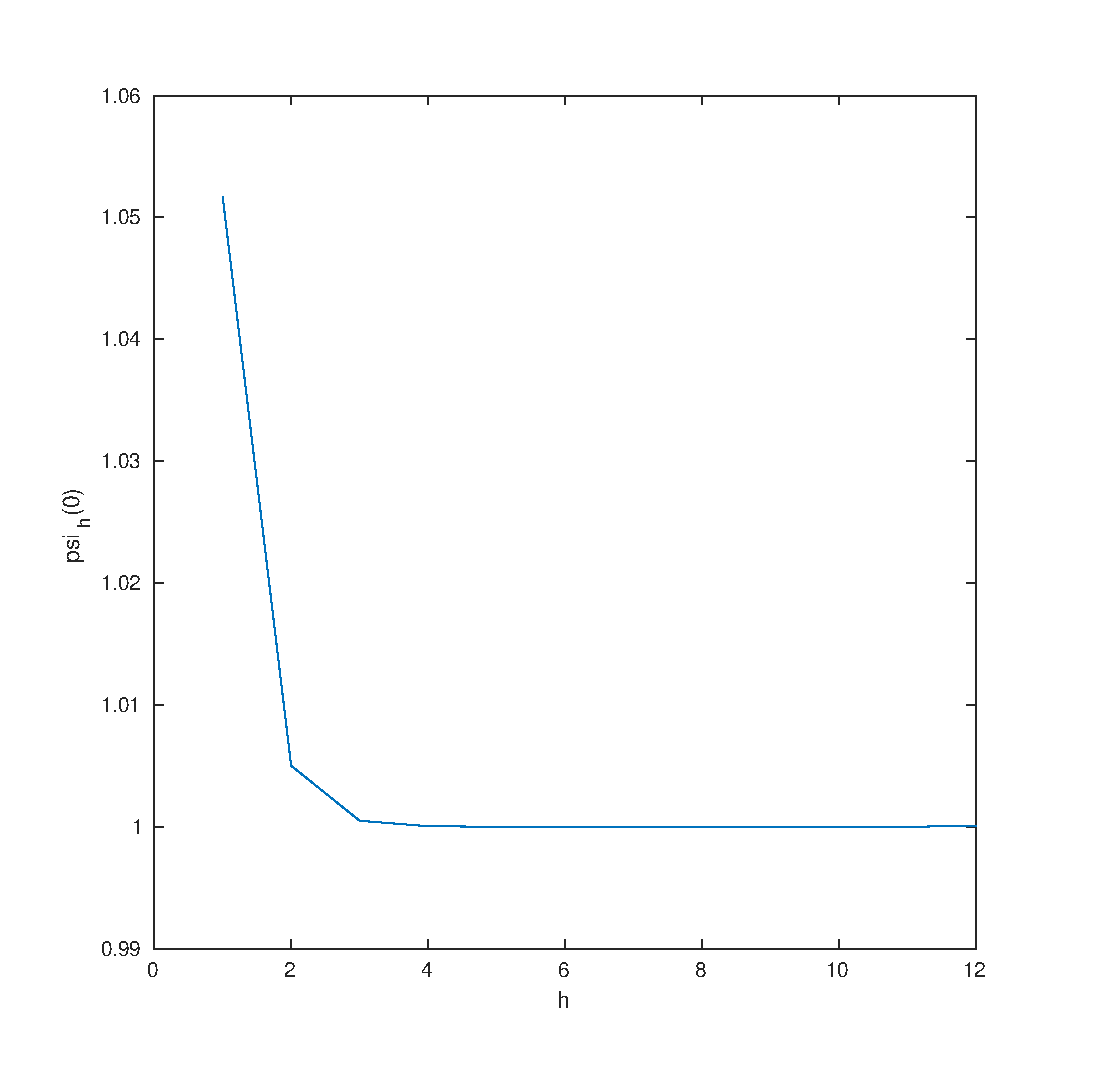
\includegraphics[width=\textwidth]{plot/fes4.eps}
\end{figure}

\end{document}
